\documentclass[11pt]{article}
\usepackage[margin=0.78in]{geometry}
\usepackage{amsmath,amssymb,bm,booktabs,array,multirow}
\usepackage{xcolor,graphicx,tikz}
\usetikzlibrary{arrows.meta,positioning,shapes.geometric}
\usepackage[most]{tcolorbox}
\usepackage{enumitem,fancyhdr,hyperref,microtype}
\graphicspath{{../../results/mahdavi_deeponet/}}
\definecolor{navy}{HTML}{17365D}
\definecolor{blue}{HTML}{2F75B5}
\definecolor{teal}{HTML}{2A9D8F}
\definecolor{gold}{HTML}{E9A23B}
\definecolor{red}{HTML}{C44536}
\definecolor{lightblue}{HTML}{EAF3F8}
\definecolor{lightgold}{HTML}{FFF6E6}
\hypersetup{colorlinks=true,linkcolor=navy,urlcolor=blue,citecolor=navy}
\pagestyle{fancy}\fancyhf{}
\lhead{M\&I-ENG 690A -- AI in Fluid Mechanics}\rhead{Week 9 Extension}\cfoot{\thepage}
\setlength{\headheight}{14pt}
\setlist{itemsep=3pt,topsep=4pt}
\newtcolorbox{learningbox}{colback=lightblue,colframe=blue,title=Learning checkpoint,fonttitle=\bfseries}
\newtcolorbox{warningbox}{colback=lightgold,colframe=gold,title=Scientific boundary,fonttitle=\bfseries}
\newtcolorbox{evidencebox}{colback=white,colframe=navy,title=Evidence gate,fonttitle=\bfseries}
\newtcolorbox{decisionbox}{colback=teal!6,colframe=teal,title=Decision rule,fonttitle=\bfseries}
\newcommand{\RelLtwo}{\varepsilon_{L_2}}
\newcommand{\Kn}{\mathrm{Kn}}

\begin{document}
\hypersetup{pageanchor=false}
\begin{titlepage}
\centering\vspace*{0.8cm}
{\color{navy}\rule{\textwidth}{2pt}}\\[0.45cm]
{\Huge\bfseries Rarefied-Flow CFD and\\[0.16cm]DeepONet Case Studies\par}
\vspace{0.32cm}{\Large Micro-Step and Micro-Nozzle: from DSMC verification to held-out fields\par}
\vspace{0.32cm}{\large Week 9 Extension Lecture Notes\par}
\vspace{0.48cm}{\color{navy}\rule{\textwidth}{2pt}}\\[0.8cm]
{\Large M\&I-ENG 690A -- AI in Fluid Mechanics\par}
\vspace{0.2cm}{\large Summer 2026\par}
\vfill
\begin{tcolorbox}[colback=lightblue,colframe=blue,width=0.92\textwidth]
\textbf{Central question.} How do we establish credible DSMC labels first, then train and test a neural operator without confusing flow-solver verification, data integrity, and surrogate error?
\end{tcolorbox}
\vfill{\large Instructor: Ehsan Roohi\par}
\end{titlepage}

\hypersetup{pageanchor=true}
\pagenumbering{roman}
\tableofcontents\newpage
\pagenumbering{arabic}

\section{Position in the Course}
Week 9 joins two 2026 Roohi--Mahdavi studies to the course's earlier DSMC,
operator-learning, and validation material. The micro-step varies rarefaction
or step height; the micro-nozzle varies back pressure and, in the article, the
throat location. The numerical solver and the learned operator have separate
questions, evidence, and acceptance gates.

\begin{learningbox}
By the end of the lecture and two laboratories, a student should be able to:
\begin{enumerate}
\item summarize the DSMC move--index--collide--boundary--sample algorithm;
\item design particle, mesh, time-step, sampling, and conservation checks;
\item write the branch--trunk form of DeepONet and a POD-trunk variant;
\item split complete physical cases into development, validation, and held-out groups;
\item interpret global, local-zone, centerline, and full-field errors together;
\item regenerate the FlowMLLab back-pressure figures from public DSMC fields; and
\item state which article results are references and which are new executable results.
\end{enumerate}
\end{learningbox}

\subsection{The three evidence layers}
\begin{center}
\begin{tabular}{p{0.22\textwidth}p{0.34\textwidth}p{0.32\textwidth}}
\toprule
Layer & Question & Minimum evidence \\
\midrule
DSMC solver & Does the particle calculation approximate the intended kinetic problem? & $\Delta x/\lambda$, $\Delta t/\tau_c$, particles/cell, sampling uncertainty, boundaries, conservation \\
Dataset & Are the retained arrays the intended solver outputs? & source revision, hashes, units, grid, finite values, case metadata \\
Neural operator & Does the fitted map generalize to new physical cases? & case-wise split, frozen selection, baselines, local and global errors, failure cases \\
\bottomrule
\end{tabular}
\end{center}

\clearpage
\section{DSMC as an Independent Computational Experiment}
For a dilute gas, the Knudsen number compares a molecular mean free path to a
characteristic length,
\begin{equation}
\Kn=\frac{\lambda}{L}.
\end{equation}
When continuum closure becomes questionable, DSMC advances representative
particles while separating free motion and binary collisions over a short time
step.

\subsection{One DSMC time step}
\begin{center}
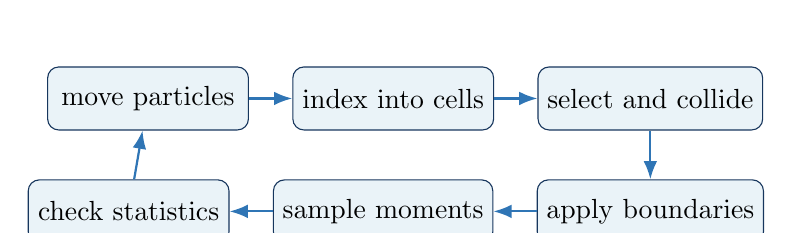
\begin{tikzpicture}[node distance=0.62cm and 0.55cm,>=Latex]
\tikzset{box/.style={draw=navy,rounded corners,minimum width=2.55cm,minimum height=0.8cm,align=center,fill=lightblue}}
\node[box] (m) {move particles};
\node[box,right=of m] (i) {index into cells};
\node[box,right=of i] (c) {select and collide};
\node[box,below=of c] (b) {apply boundaries};
\node[box,left=of b] (s) {sample moments};
\node[box,left=of s] (q) {check statistics};
\draw[->,thick,blue] (m)--(i);
\draw[->,thick,blue] (i)--(c);
\draw[->,thick,blue] (c)--(b);
\draw[->,thick,blue] (b)--(s);
\draw[->,thick,blue] (s)--(q);
\draw[->,thick,blue] (q)--(m);
\end{tikzpicture}
\end{center}

\begin{enumerate}
\item \textbf{Move:} update position from molecular velocity during $\Delta t$.
\item \textbf{Boundary interaction:} process inlet, outlet, symmetry, and wall reflection/accommodation.
\item \textbf{Index:} place particles in collision cells or subcells.
\item \textbf{Collide:} choose candidate pairs; an NTC scheme accepts pairs according to relative speed and cross section.
\item \textbf{Sample:} after a transient, accumulate number, momentum, and energy moments over many statistically correlated steps.
\end{enumerate}

The familiar design rules are local: collision cells should resolve the local
mean free path, the time step should resolve the local mean collision time,
and particle count and sample duration must make the uncertainty acceptable in
the specific observable of interest.

\begin{evidencebox}
A credible CFD/DSMC submission reports at least two spatial resolutions, two
time steps, particles per cell, sampling length, independent seeds or block
statistics, wall model, inlet/outlet treatment, mass balance, and uncertainty
on the final comparison quantities. A smooth contour is not a convergence test.
\end{evidencebox}

\clearpage
\section{From Fields to Operators}
A parameter-to-field operator predicts the response at a query coordinate
$\bm y$ for a physical input $\bm p$. A standard DeepONet writes
\begin{equation}
\widehat{G}(\bm p)(\bm y)=\sum_{k=1}^{r}b_k(\bm p)t_k(\bm y)+b_0.
\end{equation}
The branch produces coefficients $b_k$; the trunk produces coordinate features
$t_k$. In a POD--DeepONet, the trunk is a set of POD modes learned from the
development fields, while a neural branch predicts their coefficients.

\subsection{Case-wise experimental design}
For the nozzle back-pressure study, FlowMLLab uses
\begin{align}
\mathcal D_{\rm dev}&=\{15,18,19,20,22,23,24,26,27,28,29,33\}\ \mathrm{kPa},\\
\mathcal D_{\rm test}&=\{16,25,30\}\ \mathrm{kPa}.
\end{align}
Two full-field baselines are compared inside $\mathcal D_{\rm dev}$:
physical-coordinate interpolation and interpolation after aligning row-wise
density-compression surfaces. Alignment is selected per output only when it
reduces mean shock-window error and increases mean global error by at most two
percentage points. The held-out fields are evaluated after that rule and all
metric definitions are fixed.

For a reference field $q$ and prediction $\widehat q$,
\begin{equation}
\RelLtwo(q,\widehat q)=
\frac{\lVert\widehat q-q\rVert_2}{\lVert q\rVert_2}\times100\%.
\end{equation}
This metric must be supplemented by localized error, shock position, reverse-
flow topology, conservation, and uncertainty of the DSMC reference.
FlowMLLab therefore also reports a row-wise window within $\pm3\delta_j$ of the
reference shock and a density-gradient-weighted norm with
$w=1+4|\partial\rho/\partial x|/\max|\partial\rho/\partial x|$. The reference
shock is used only to score a completed prediction; the predicted aligned
coordinate comes solely from bracketing development fields.

\begin{warningbox}
Model error relative to DSMC is not DSMC error relative to the physical flow.
The first evaluates the operator against its numerical labels. The second
requires independent solver verification and external validation evidence.
\end{warningbox}

\clearpage
\section{Micro-Step: Physics and Zonal Learning}
The backward-facing micro-step creates separation, reverse flow, and
reattachment in a small region. A domain-average loss can underweight that
region. The physics-guided zonal objective is
\begin{equation}
\mathcal L_{\rm zonal}=\alpha\mathcal L_{U<0}
+(1-\alpha)\mathcal L_{U\ge0},
\end{equation}
where each regional mean is normalized by its own number of points.

FlowMLLab keeps five heights for development, H33/H58 for validation, and
H44/H67 for the held-out classroom evaluation. The validation rule selects
$\alpha=0.6$. The article and classroom figures use equal $x/H$--$y/H$
scaling; the measured data domain has $L/H\simeq5$.

The pinned article-repository inference path constructs each local input patch
from the same DSMC $U,V$ field that it reconstructs. Its stored C-DeepONet
panels are therefore target-assisted reconstruction evidence, not an
independently deployable held-out map. A nearest-sample baseline on that patch
gives 4.40\% at H44 and 6.79\% at H67, lower than the stored model's 4.92\%
and 8.23\%. The classroom model instead receives only height, coordinates, and
known geometry.

\begin{figure}[ht]
\centering
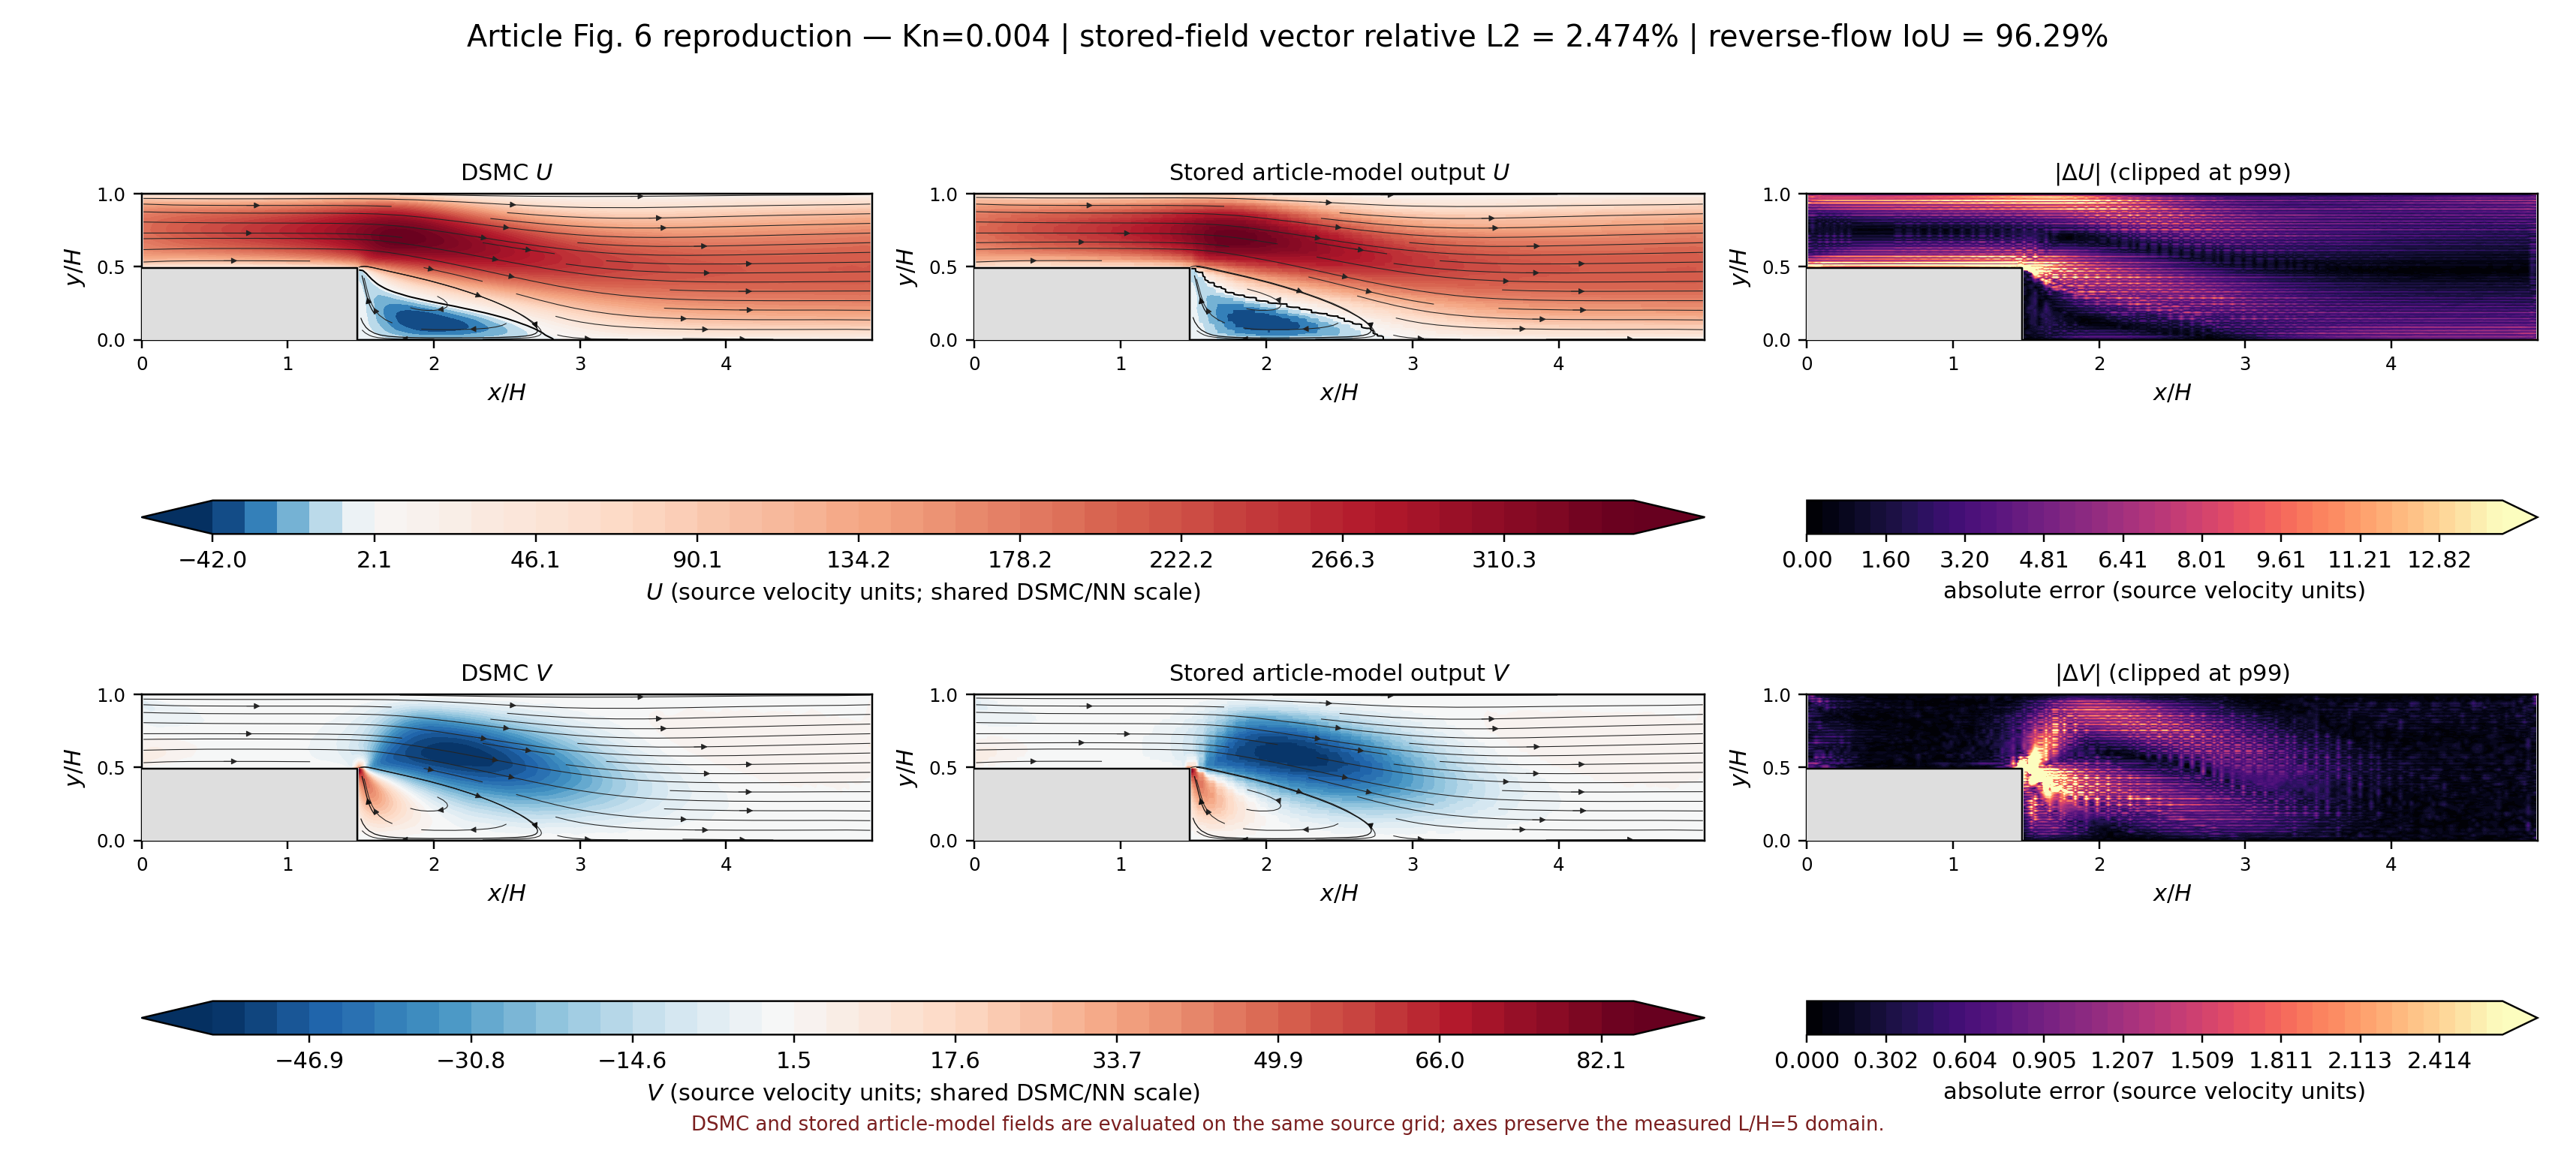
\includegraphics[width=\textwidth]{step_article_contours/article_figure_06_Kn0p004.png}
\caption{Micro-step rarefaction case at $\Kn=0.004$: DSMC, stored target-assisted article-model output, and absolute velocity error. The solid step remains masked and the field color limits are shared.}
\label{fig:step-kn}
\end{figure}

\clearpage
\section{Micro-Step: Height Variation and Local Metrics}
\begin{figure}[ht]
\centering
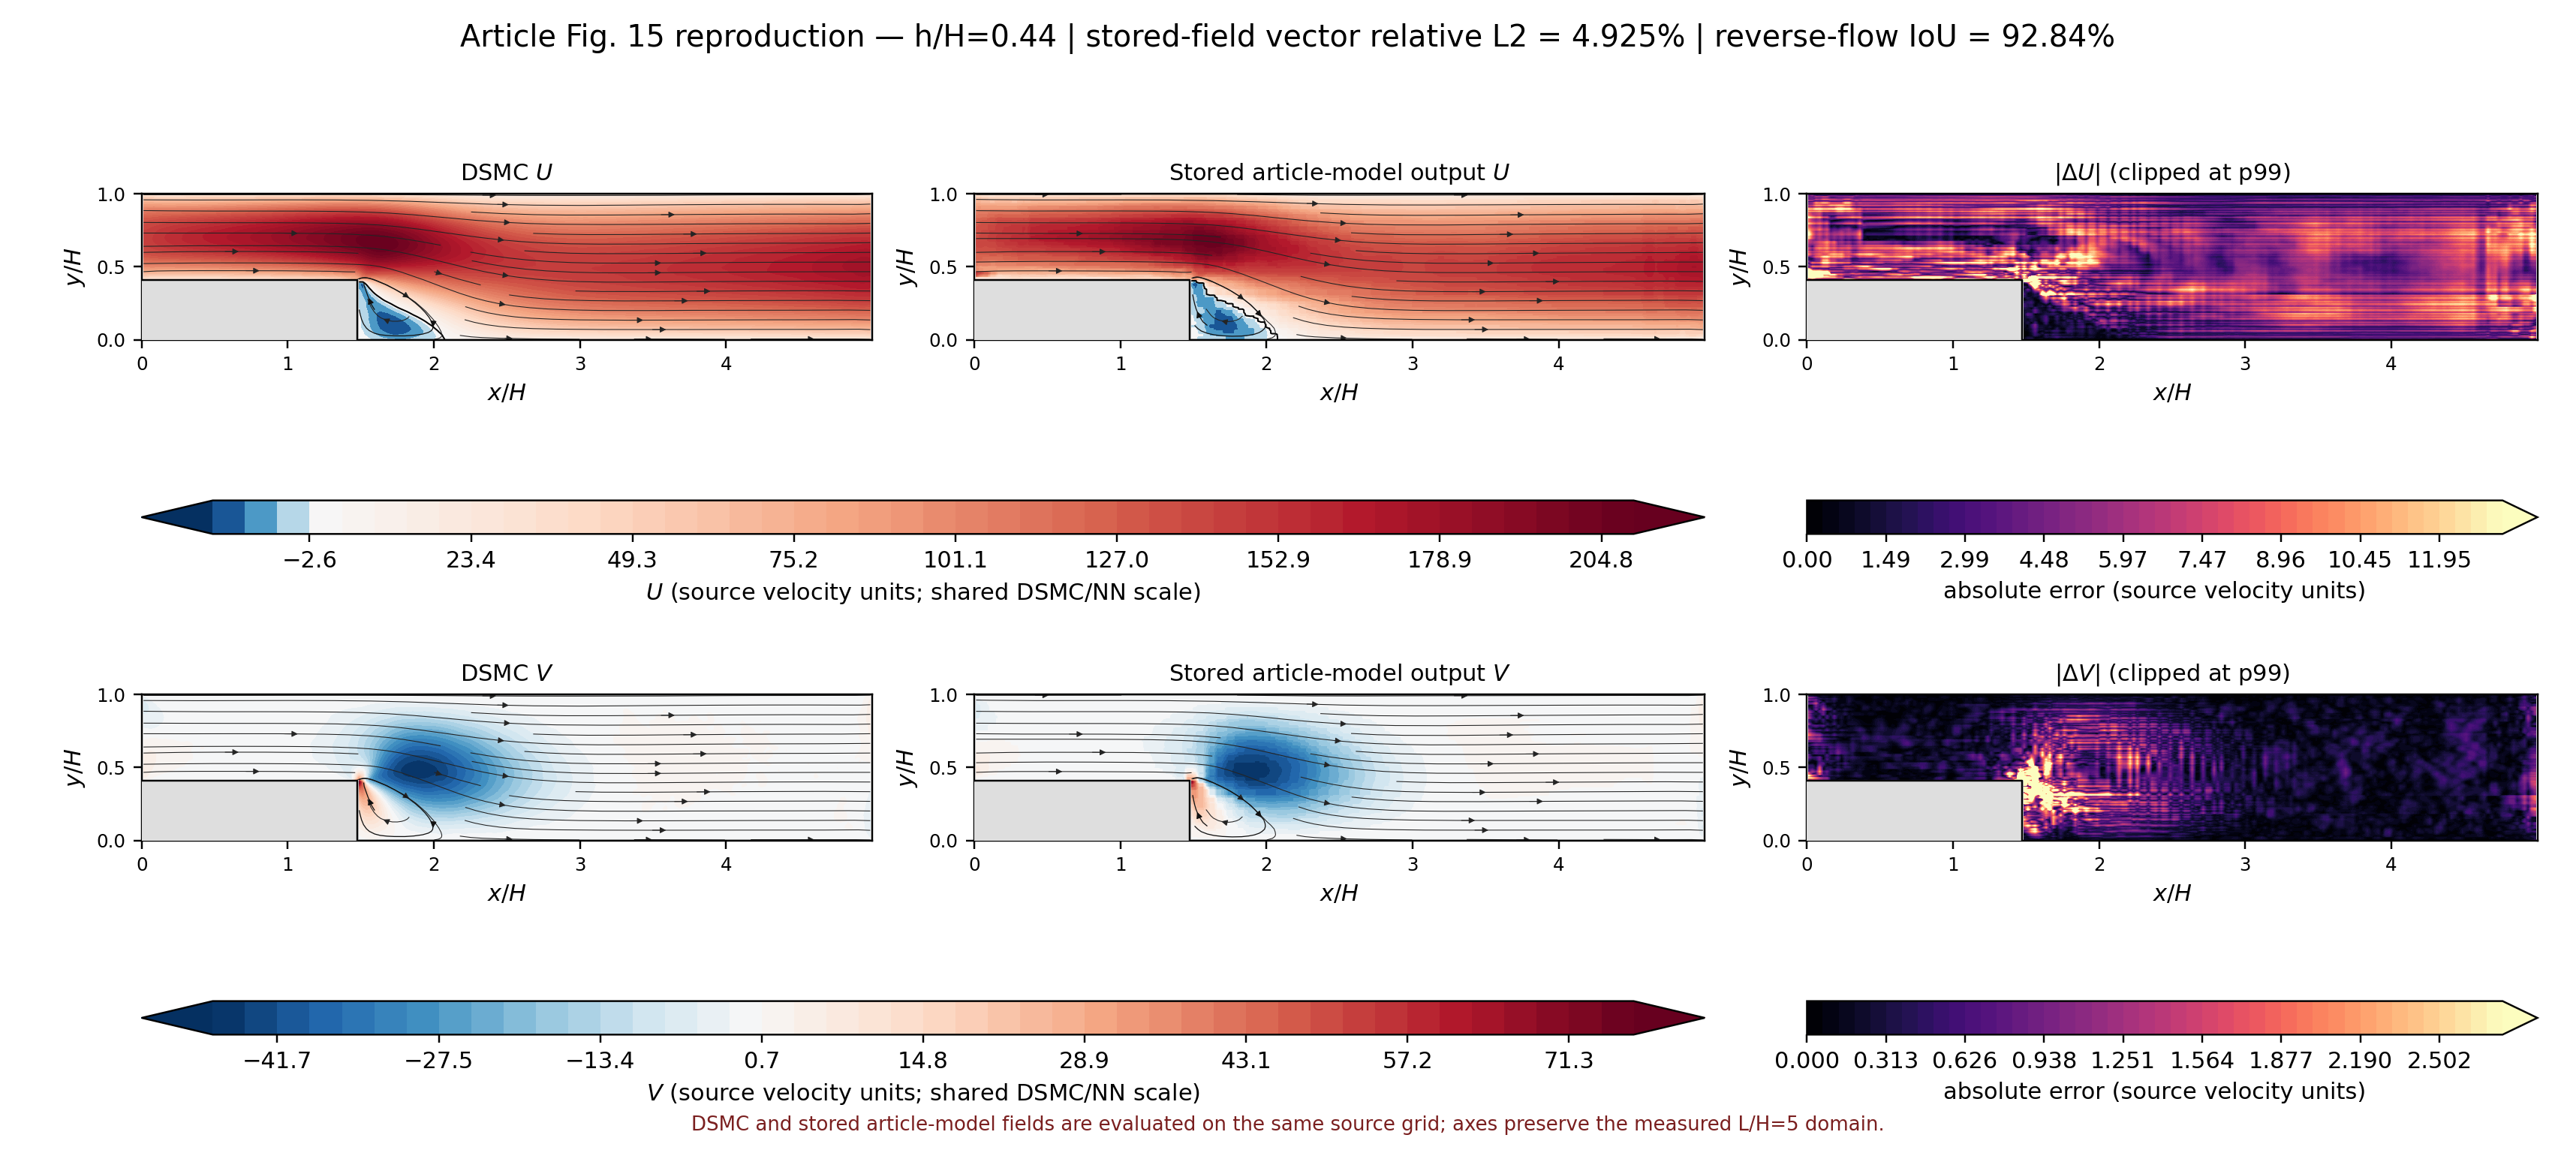
\includegraphics[width=\textwidth]{step_article_contours/article_figure_15_H44.png}
\caption{Article height-variation case H44, rebuilt on its source grid. Reverse-flow IoU and reattachment length complement the vector relative $L_2$ value.}
\label{fig:step-height}
\end{figure}

The independently trained FlowMLLab classroom model provides a second
comparison at H44/H67:
\begin{center}
\begin{tabular}{lrrrr}
\toprule
Case & Vector $L_2$ & Reverse-zone $L_2$ & Reverse-flow IoU & $L_r/L$ (DSMC/model) \\
\midrule
H44 & 9.594\% & 19.863\% & 93.27\% & 0.1199 / 0.1138 \\
H67 & 11.267\% & 33.257\% & 80.49\% & 0.1042 / 0.1149 \\
\bottomrule
\end{tabular}
\end{center}
The local improvement is purchased with a substantial global tradeoff:
unweighted-to-zonal error changes from 7.228\% to 9.594\% at H44 and from
5.934\% to 11.267\% at H67. The latter is almost a factor of two; describing
it as a modest increase would contradict the held-out table.

\begin{decisionbox}
The zonal model is accepted only if validation shows the planned reverse-flow
improvement without violating the predeclared global-error allowance. The
held-out geometries report the result; they do not select $\alpha$.
\end{decisionbox}

\clearpage
\section{Micro-Nozzle Back Pressure: New FlowMLLab Fields}
The public nozzle dataset contains 15 complete DSMC snapshots on a common
101-by-31 curvilinear grid. FlowMLLab preserves density, temperature, $U$, $V$,
Mach number, pressure, and Knudsen number. For each of the six article outputs,
physical-coordinate and shock-aligned interpolation are compared on 12
development pressures. The aligned route detects the downstream density
compression in each source-field row, interpolates its location in pressure,
translates both source rows to that predicted surface, and only then blends
them. It does not inspect the held-out target field.

\begin{figure}[ht]
\centering
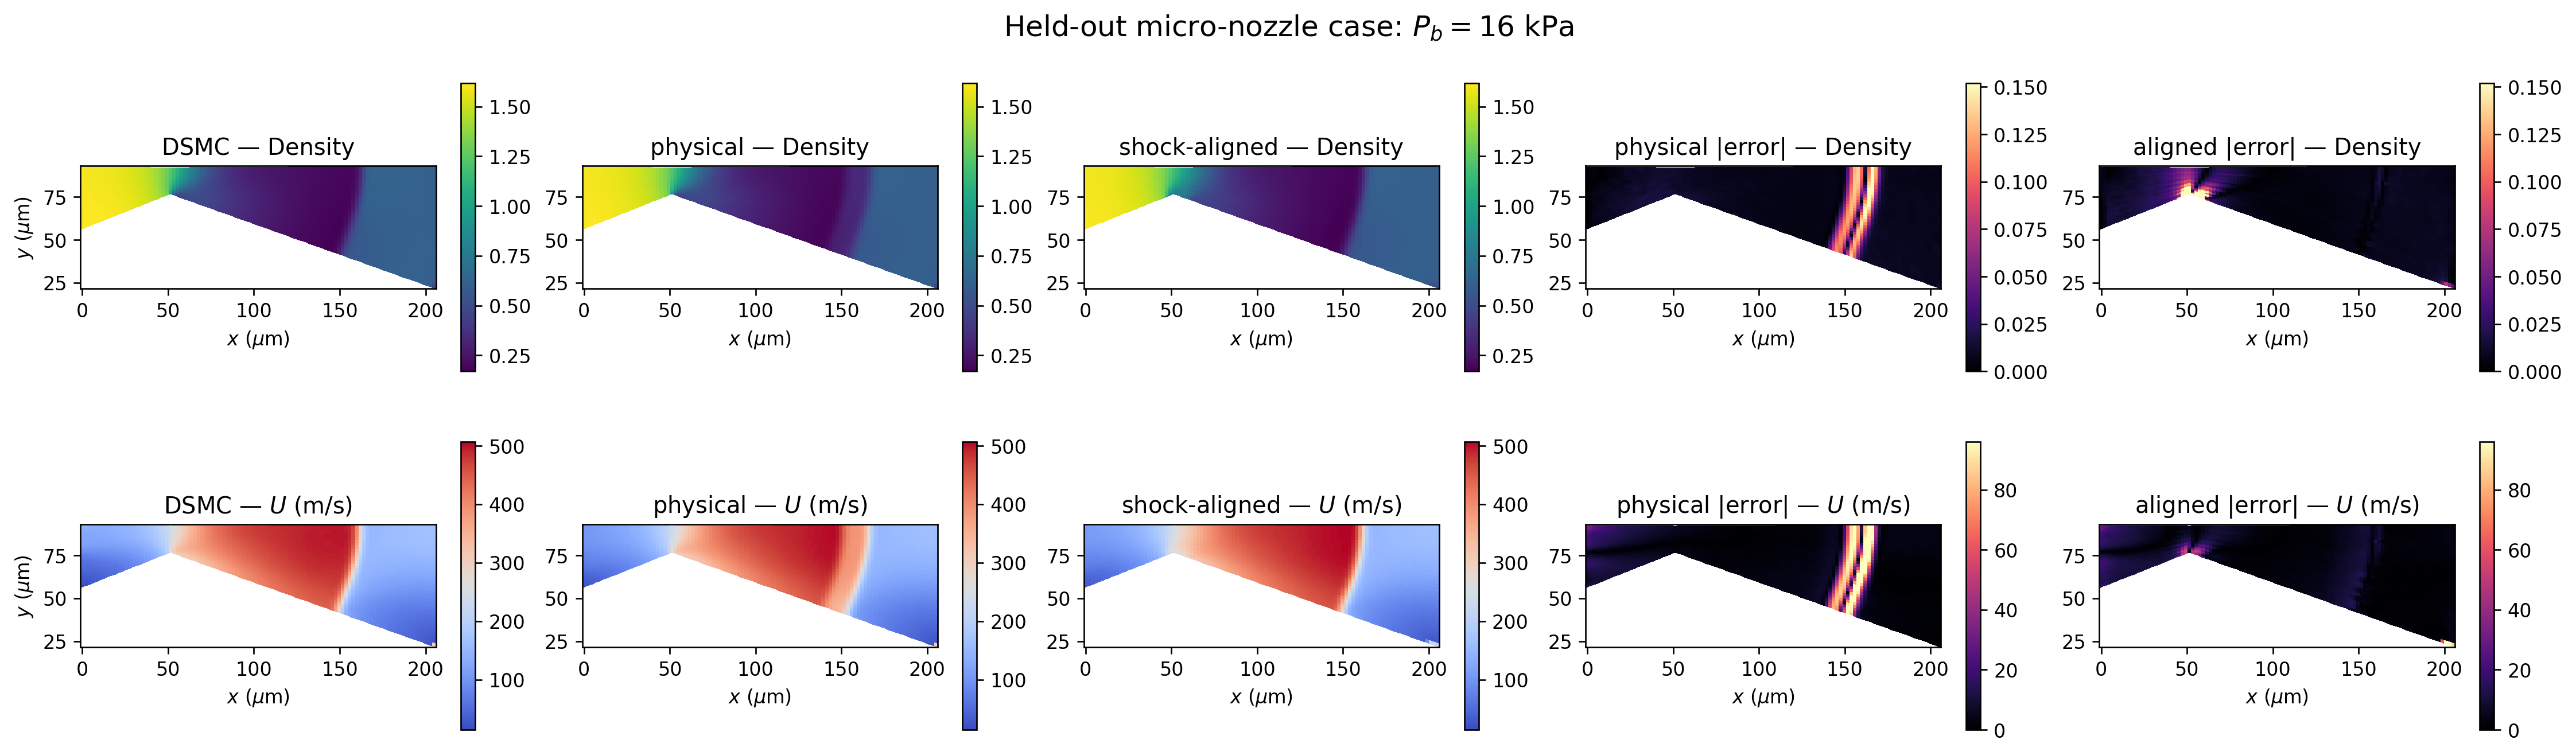
\includegraphics[width=\textwidth]{nozzle_flowmllab/nozzle_back_pressure_P16_contours.png}
\caption{Held-out $P_b=16$ kPa comparison of DSMC, physical-coordinate interpolation, and shock-aligned interpolation. Shared field and error scales expose how alignment removes most translated-shock smear in $U$ while preserving the nozzle aspect.}
\label{fig:nozzle-contour}
\end{figure}

The largest discrepancies concentrate around the translated compression/shock
region. This explains why apparently good upstream fields can coexist with a
larger global velocity or Mach error.

\clearpage
\section{Back-Pressure Profiles and Error Matrix}
\begin{figure}[ht]
\centering
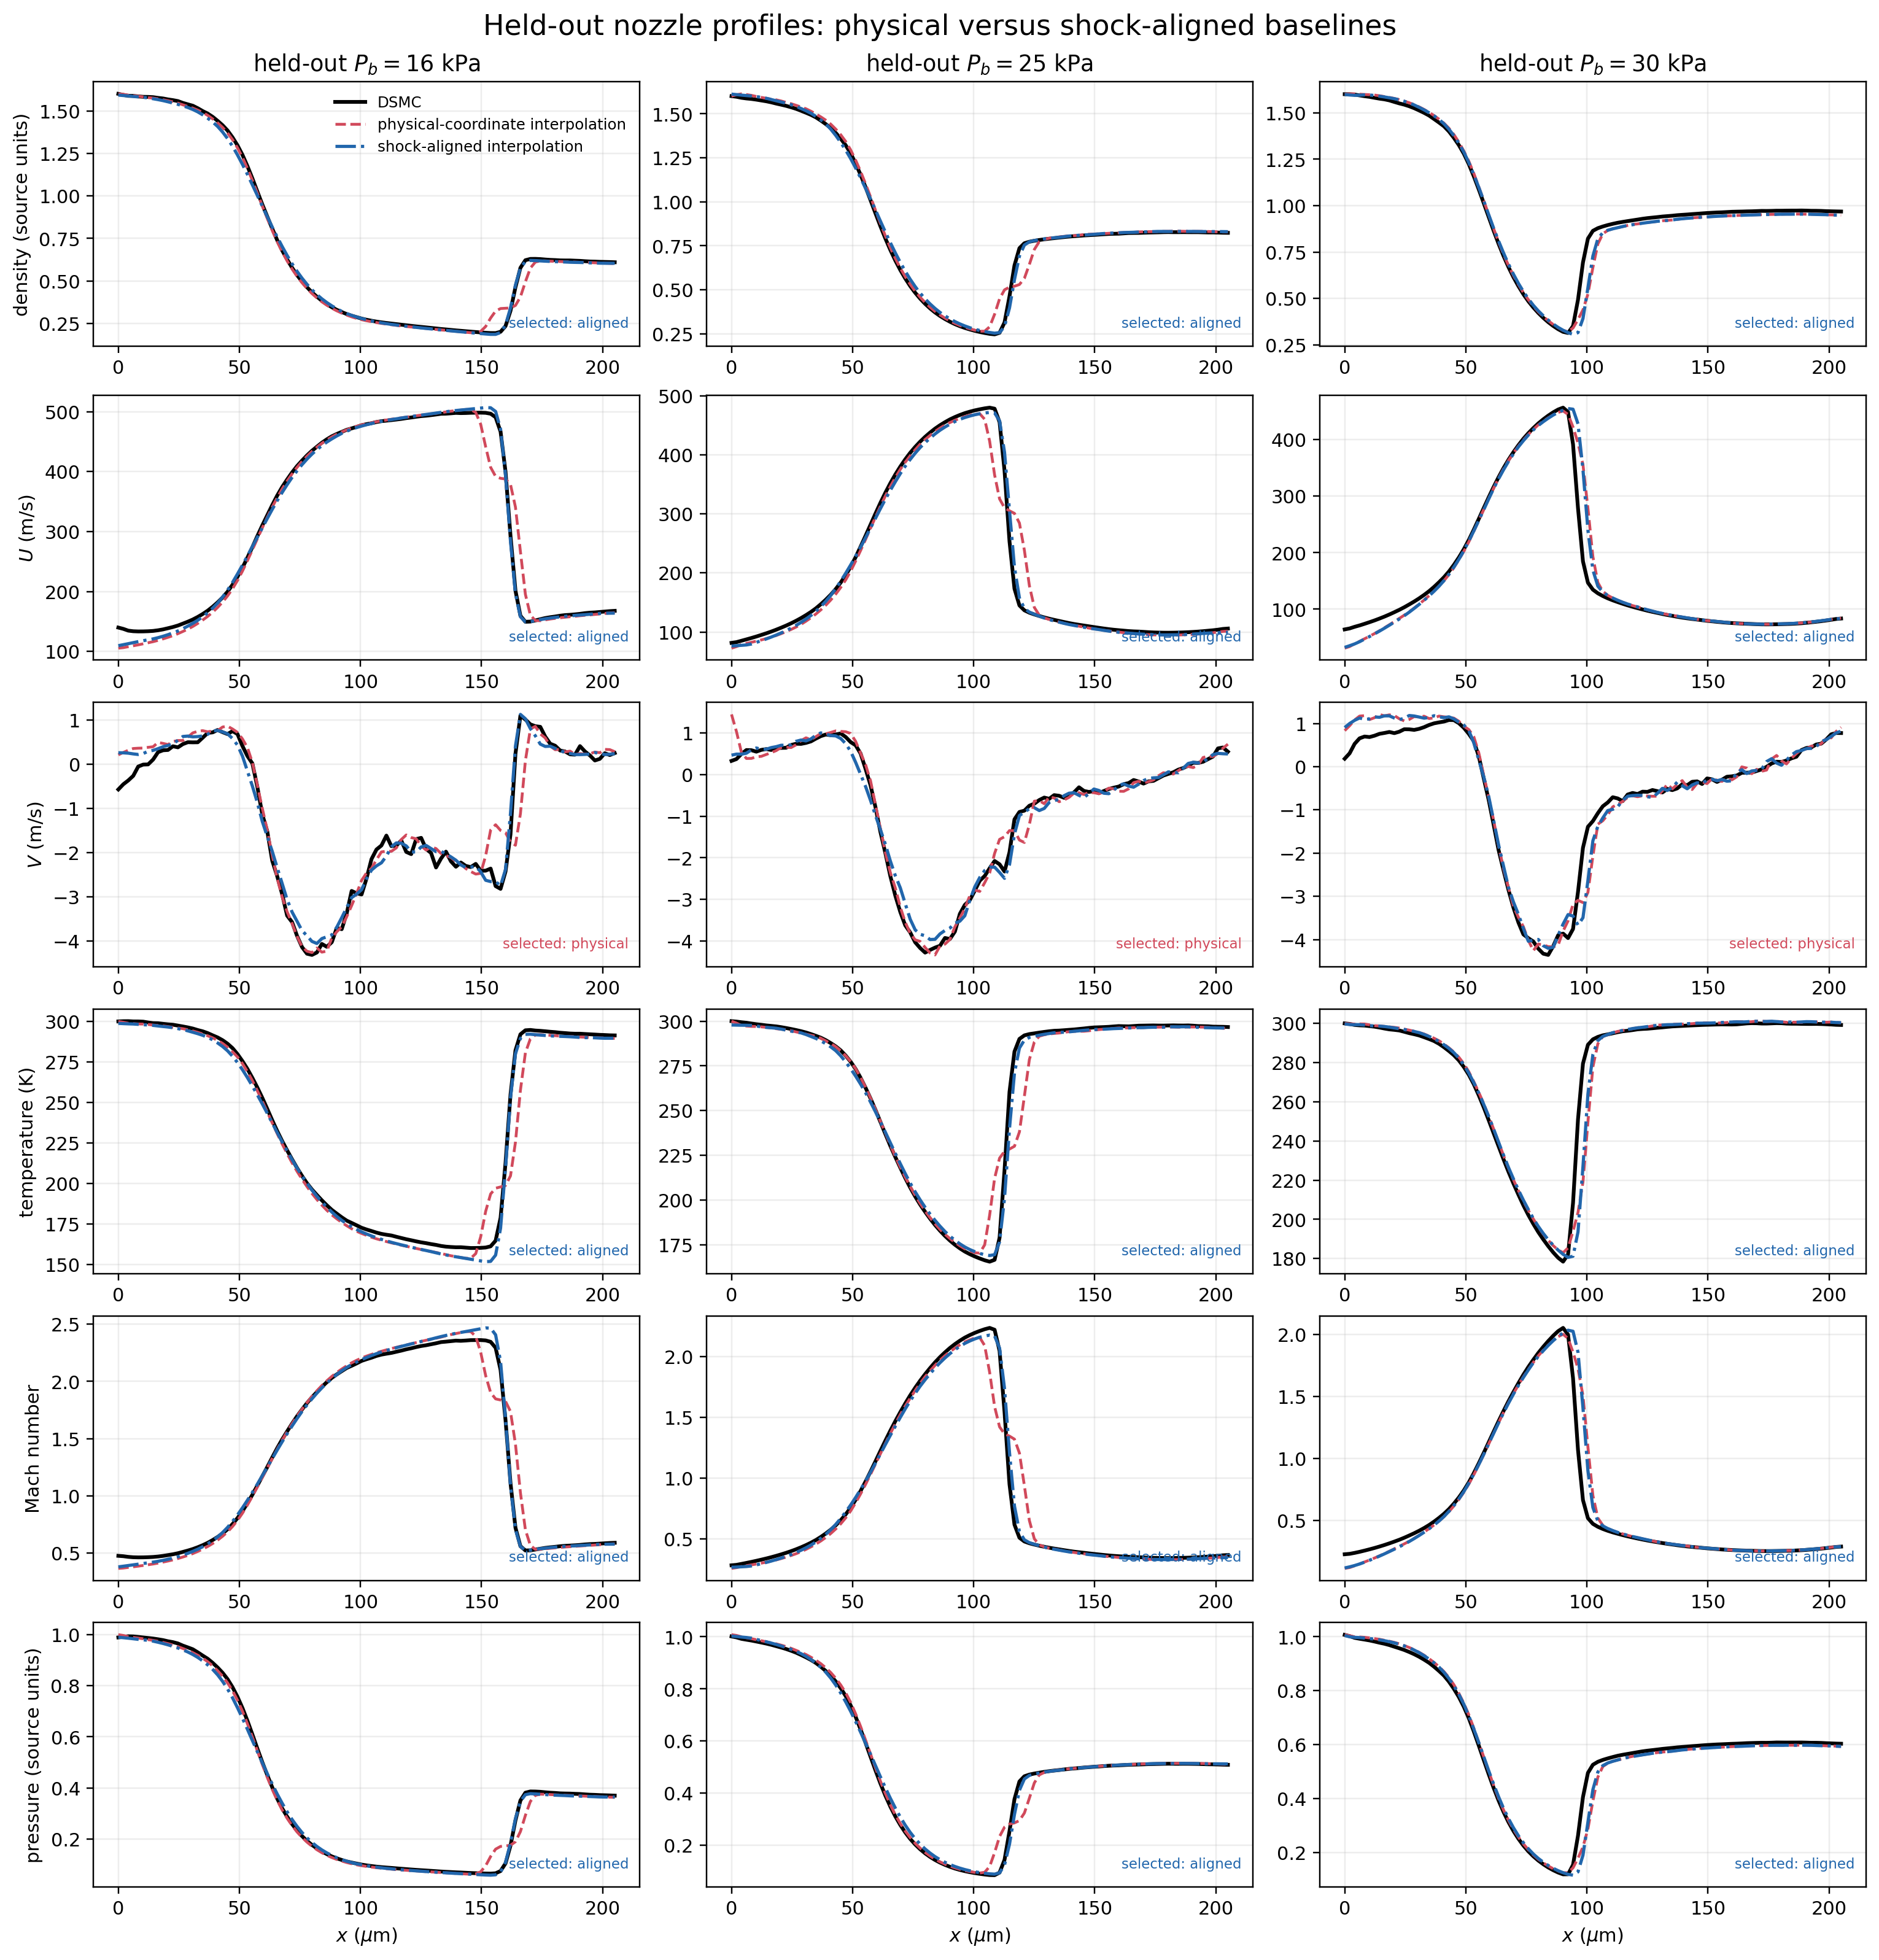
\includegraphics[width=0.78\textwidth]{nozzle_flowmllab/nozzle_back_pressure_profiles.png}
\caption{Centerline slices for both interpolation baselines at all three held-out back pressures. The selected route is frozen by development-only folds. These curves are regenerated by \texttt{qa/run\_nozzle\_field\_validation.py}.}
\label{fig:nozzle-profiles}
\end{figure}

\clearpage
\begin{figure}[ht]
\centering
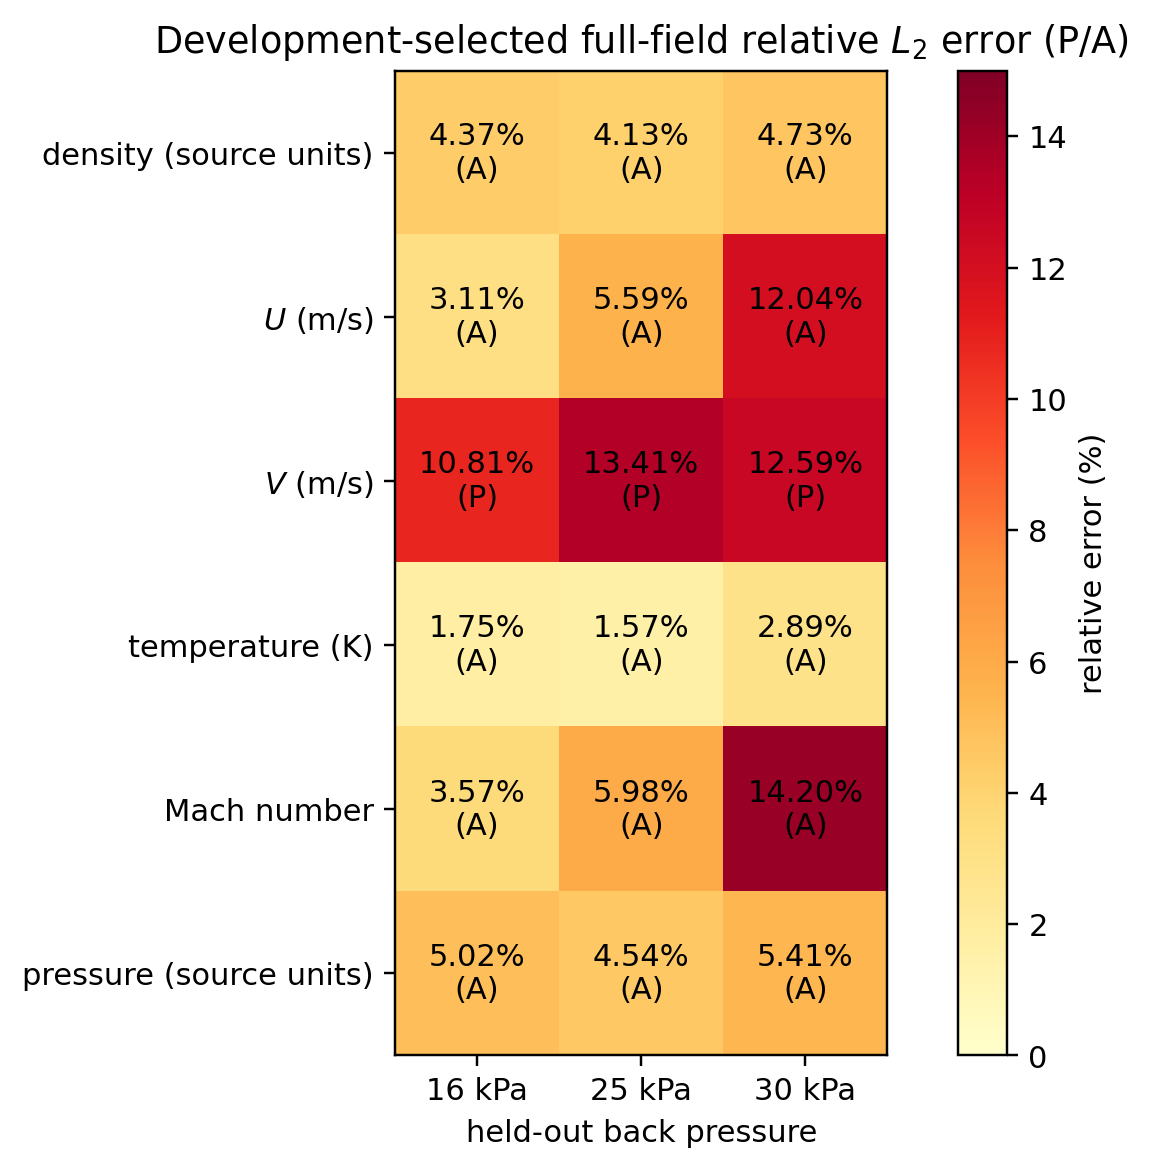
\includegraphics[width=0.68\textwidth]{nozzle_flowmllab/nozzle_back_pressure_error_summary.png}
\caption{Development-selected full-field relative $L_2$ errors. Each cell marks physical (P) or aligned (A); a single average would hide output dependence and the harder 30 kPa case.}
\label{fig:nozzle-errors}
\end{figure}

\begin{center}
\begin{tabular}{lrrr}
\toprule
Field & 16 kPa & 25 kPa & 30 kPa \\
\midrule
Density & 4.366\% & 4.130\% & 4.734\% \\
$U$ & 3.107\% & 5.586\% & 12.038\% \\
$V$ & 10.813\% & 13.409\% & 12.593\% \\
Temperature & 1.751\% & 1.572\% & 2.893\% \\
Mach number & 3.574\% & 5.984\% & 14.200\% \\
Pressure & 5.020\% & 4.539\% & 5.406\% \\
\bottomrule
\end{tabular}
\end{center}

\clearpage
\section{Shock-Centered Coordinates}
A moving sharp feature can require many linear modes in laboratory coordinates.
For detected compression location $x_s$ and width $\delta_j$, define
\begin{equation}
\xi_j=\frac{x-x_s}{\delta_j},\qquad
\widetilde\rho=\frac{\rho-\rho_R}{\rho_L-\rho_R}.
\end{equation}
Across all 15 DSMC centerlines, FlowMLLab reproduces the retained POD audit:
\begin{center}
\begin{tabular}{lrrrr}
\toprule
Coordinate & Mode 1 energy & Modes 1--2 & Modes 1--3 & Modes for 99\% \\
Physical $x$ & 78.922\% & 88.467\% & 93.762\% & 8 \\
Shock-centered $\xi_j$ & 97.986\% & 99.182\% & 99.865\% & 2 \\
\bottomrule
\end{tabular}
\end{center}

Alignment reduces representation rank; it does not by itself solve deployment.
A new case does not arrive with $x_s$. The notebook therefore evaluates a
pressure-to-shock-location component separately and retains the non-monotone
22 kPa detection as a diagnostic rather than silently deleting it.

\begin{learningbox}
Ask two questions about every learned coordinate transform: (1) how is it
estimated for a new input? (2) how does its uncertainty propagate into the
reconstructed physical field?
\end{learningbox}

\clearpage
\section{Throat-Location Variation: Reproduction Boundary}
The article also studies a geometry branch in which $x_{\rm throat}/L$ varies.
The training locations are
\[
0.10,\ 0.15,\ 0.20,\ 0.25,\ 0.35,\ 0.45,\ 0.55,
\]
and the reported held-out location is $0.30$. The article reports centerline errors of
4.07\% for density, 9.78\% for $U$, 10.85\% for Mach number, and 4.82\% for
pressure.

\begin{figure}[ht]
\centering
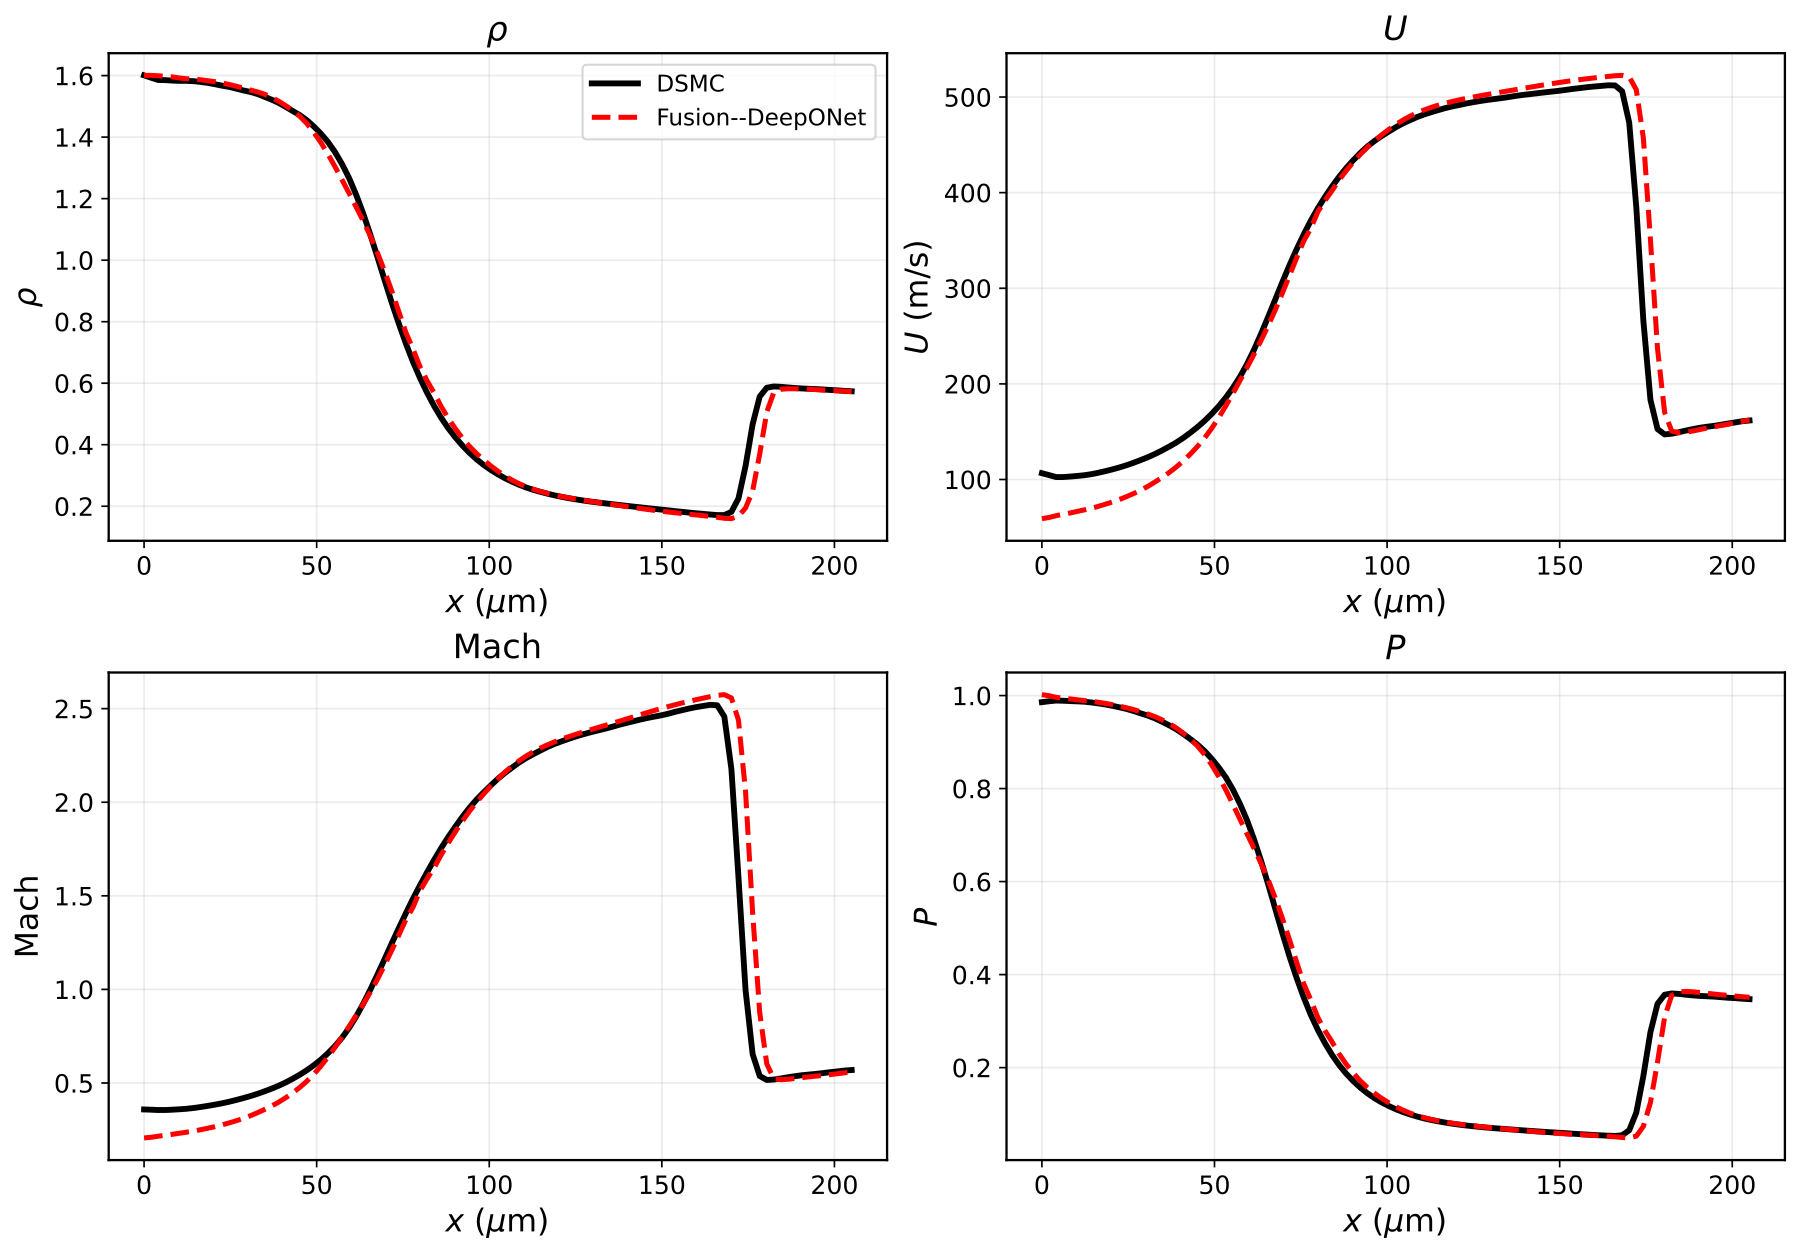
\includegraphics[width=0.92\textwidth]{nozzle_article_figures/nozzle_throat_X030_profiles.png}
\caption{Published throat-location centerline comparison at $x_{\rm throat}/L=0.30$, reproduced here as a literature reference under CC BY 4.0. It is not a FlowMLLab-generated field. Source: Roohi and Mahdavi, 2026, arXiv:2605.12723, Fig.~20.}
\label{fig:throat-reference}
\end{figure}

\begin{warningbox}
The public reproducibility repository presently contains the 15-case
back-pressure DSMC sweep, but not the throat-geometry DSMC sweep or its trained
checkpoint. Consequently, FlowMLLab regenerates the back-pressure result from
code and treats the throat plot only as a cited reference. A full throat rerun
requires publication of those geometry-indexed fields.
\end{warningbox}

\clearpage
\section{Laboratory Workflow and Assessment}
\subsection{Lab 1: micro-step}
\begin{enumerate}
\item verify hashes, row counts, units, masks, and equal physical aspect;
\item inspect one DSMC height field and identify separation and reattachment;
\item fit the coordinate baseline on development geometries;
\item select $\alpha$ using H33/H58 only;
\item evaluate H44/H67 using global, reverse-zone, IoU, and $L_r$ metrics; and
\item compare the independently trained contours with the retained article cases.
\end{enumerate}

\subsection{Lab 2: micro-nozzle}
\begin{enumerate}
\item verify the 15 public DSMC files and their full-field derivative;
\item detect $x_s$, reproduce physical versus aligned density POD, and inspect 22 kPa;
\item freeze the 12/3 pressure split, two baselines, local metrics, and global guardrail;
\item run \texttt{qa/run\_nozzle\_field\_validation.py};
\item interpret every row of the 6-by-3 error matrix and the 16 kPa contour; and
\item propose the additional data package required for the throat study.
\end{enumerate}

\subsection{Recommended grading evidence}
\begin{center}
\begin{tabular}{p{0.28\textwidth}p{0.58\textwidth}}
\toprule
Category & Required evidence \\
\midrule
DSMC verification plan & spatial/time/particle/sampling studies, wall model, conservation, uncertainty \\
Data integrity & source commit, hashes, units, coordinates, masks, case table \\
Selection discipline & development/validation/held-out cases and frozen rule \\
Field fidelity & full-field and local errors, topology or shock position, equal-aspect figures \\
Interpretation & one success, one failure, and one next numerical experiment \\
Reproducibility & restart-and-run notebook plus machine-readable metrics and figure manifest \\
\bottomrule
\end{tabular}
\end{center}

\clearpage
\section{Takeaways}
\begin{enumerate}
\item DSMC labels must be verified as a particle calculation independently of any neural model.
\item Complete physical cases, not shuffled spatial points, define the experimental split.
\item Zonal metrics expose micro-step recirculation behavior hidden by a domain average.
\item Shock alignment compresses the nozzle snapshot family from eight to two density modes at 99\% energy.
\item The selected interpolation baseline keeps every held-out full-field error below 14.21\%, but this is baseline evidence, not a regenerated DeepONet claim.
\item A cited article plot and a code-regenerated result are different evidence and must remain labelled accordingly.
\end{enumerate}

\begin{decisionbox}
The next defensible software increment is a published throat-geometry DSMC
archive with the same provenance, case metadata, full fields, and verification
records as the pressure sweep. Only then should the throat operator be trained,
selected, and evaluated in FlowMLLab.
\end{decisionbox}

\section*{Primary sources}
\begin{itemize}
\item E. Roohi and A. Mahdavi, ``Analysis of the rarefied flow at micro-step using a DeepONet surrogate model with a physics-guided zonal loss function,'' \emph{Microfluidics and Nanofluidics} 30:44 (2026), \href{https://doi.org/10.1007/s10404-026-02899-8}{doi:10.1007/s10404-026-02899-8}.
\item E. Roohi and A. Mahdavi, ``Shock-Centered Low-Rank Structure and Neural-Operator Representation of Rarefied Micro-Nozzle Flows,'' \emph{Physics of Fluids} 38, 082008 (2026), \href{https://doi.org/10.1063/5.0343101}{doi:10.1063/5.0343101}.
\item Public nozzle DSMC/POD package: \href{https://github.com/Ehsan-Roohi/roohi-nozzle-pod-reproducibility}{github.com/Ehsan-Roohi/roohi-nozzle-pod-reproducibility}, pinned in FlowMLLab at commit \texttt{e1b234b}.
\end{itemize}

\end{document}
